% !TeX TXS-program:compile = txs:///pythonlualatex

\documentclass[a4paper,11pt]{article}
\usepackage[pythontex]{cp-base}
\graphicspath{{./graphics/}}
%variables
\donnees[%
	typedoc=CHAPITRE~,
	numdoc=2,
	classe=1\up{ère} 2M2,
	matiere={[SPÉ.MATHS]},
	annee=2021,
	titre=Suites numériques
	]

%formatage
\author{Pierquet}
\title{\nomfichier}
\hypersetup{pdfauthor={Pierquet},pdftitle={\nomfichier},allbordercolors=white,pdfborder=0 0 0,pdfstartview=FitH}
%divers
\lhead{\entete{\matiere}}
\chead{\entete{\lycee}}
%\rhead{\entete{\classe{} - \mois{} \annee}}
\rhead{\entete{\classe{} - Chapitre \thepart}}
\lfoot{\pied{\matiere}}
\cfoot{\logolycee{}}
\rfoot{\pied{\numeropagetot}}

\begin{document}

\pagestyle{fancy}

\part{CH02 - Suites numériques}

\section{Définitions}

\subsection{Vocabulaire et notations}

\begin{cdefi}
Une \textbf{suite numérique} est une liste (infinie) de nombres, appelés \textbf{termes}, qui sont ordonnés et numérotés.

Le premier terme d'une suite $u$ se note $u_1$, le suivant $u_2$, \dots{} et plus généralement, le terme de rang $n$ , appelé aussi \textbf{terme d'indice $n$}, se note $u_n$.

L'ensemble de tous ces termes, qui constitue la suite, est noté $u$ ou plus souvent $(u_n)$.
\end{cdefi}

\begin{crmq}[s]
\begin{itemize}[leftmargin=*,topsep=0pt,parsep=0pt,partopsep=0pt]
	\item Une suite est en fait une fonction définie sur l'ensemble $\N$ des entiers naturels : à chaque entier $n$ elle fait correspondre une et une seule image $u_n$
	\item Comme l'ensemble $\N$ a pour plus petit élément 0, il est très courant de noter $u_0$ le premier terme de la suite. En fonction des situations, on choisira de démarrer à $u_1$ ou $u_0$ (ou même encore d'autres indices) suivant ce qui sera le plus naturel.
\end{itemize}
\end{crmq}

\subsection{Différents modes de définition}

\begin{ccadre}
Il existe plusieurs modes de génération d'une suite :
\begin{itemize}[leftmargin=*]
	\item Avec une formule de \emph{récurrence} : Les termes sont définis \emph{de proche en proche}. Une formule de récurrence explique comment passer d'un terme au suivant. C'est en général une relation entre deux termes consécutifs $u_n$ et $u_{n+1}$. Dans ce cas, il faut également préciser la valeur et l'indice du premier terme de la suite. Pour calculer un terme d'une suite définie par récurrence, il faut \textit{a priori} d'abord calculer tous les termes précédents.
	\item Avec une formule \emph{explicite} : Les termes ne dépendent que de leur rang $n$. On peut calculer n'importe quel terme directement. On se rapproche davantage de la notion de fonction qu'on a l'habitude d'utiliser. $u_n$ est défini à partir d'une formule dépendant de $n$.
\end{itemize}
\end{ccadre}

\begin{cmethode}
Pour bien comprendre et étudier une suite, il est impératif de savoir avant tout si la suite est une suite \textbf{récurrente} ou une suite \textbf{explicite}. Les techniques d'étude ne seront pas les mêmes dans les deux cas.
\end{cmethode}

\begin{cexemple}[s]
\begin{itemize}[leftmargin=*]
	\item La suite $(u_n)$ définie par $\begin{cases}u_0=5& \\u_{n+1}=2u_n-3& \mbox{pour tout } n\in\N 		\end{cases}$ est une suite \textbf{récurrente}.
	
	La formule explique que pour déterminer un terme de la suite, on prend le précédent et on le multiplie par 2 puis on soustrait 3 au résultat, et ainsi de suite en démarrant avec le nombre 5.
	
	$\textcolor{blue}{u_0}=\textcolor{blue}{5}$ d'après l'énoncé.
	
	$\textcolor{red}{u_1}=2\textcolor{blue}{u_0}-3=2\times\textcolor{blue}{5} -3=\textcolor{red}{7} \text{ et } \textcolor{green}{u_2}=2\times \textcolor{red}{7}-3=\textcolor{green}{11} \text{ et } u_3=2\times11-3=19$ etc
	\item La suite $(v_n)$ définie par $v_n=2^n-5 $ pour tout $n \in \N$ est une suite \textbf{explicite}.
	
	La formule explique que, pour calculer le $n$-ième terme de cette suite, on élève 2 à la puissance $n$ puis on soustrait 5. Il n'est pas nécessaire de connaître le terme précédent pour le calculer, seul son \textbf{rang} est nécessaire.
	
	$v_{\textcolor{blue}{0}}=2^{\textcolor{blue}{0}}-5=1-5=-4 \text{ et } v_{\textcolor{red}{1}}=2^{\textcolor{red}{1}}-5=2-5=-3 \text{ et } v_{\textcolor{green}{7}}=2^{\textcolor{green}{7}}-5=128-5=123$ etc
\end{itemize}
\end{cexemple}

\subsection{Méthodes de calculs}

\begin{ccalco}
À la calculatrice, on peut utiliser la touche \ccalg{Ans} pour calculer les termes consécutifs de la suite :
\begin{center}
	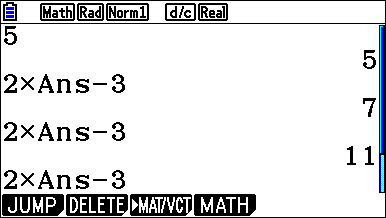
\includegraphics[height=2.25cm]{chap02_suites_ans_90}~~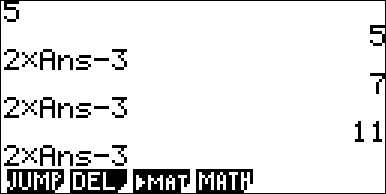
\includegraphics[height=2.25cm]{chap02_suites_ans_35}
\end{center}
\end{ccalco}

\begin{clog}
On peut utiliser un \csheet{tableur} pour calculer les termes d'une suite (explicite ou non), grâce aux références des cellules puis à la \csheet{poignée de recopie} :

\smallskip

\begin{tikzpicture}
	\tableur[4]{A-B}
	\celtxt*[c]{A}{1}{$n$}
	\celtxt*[c]{B}{1}{$u(n)$}
	\celtxt[c]{A}{2}{0}
	\celtxt[c]{A}{3}{1}
	\celtxt[c]{A}{4}{2}
	\selecCell{B}{2}
	\draw[thick,ForestGreen,<-,>=latex'] ($(cellB-2.center)+(4pt,0)$) to [bend right=5] ($(cellB-2)+(2.25,-0.25)$) node[right] {formule explicite en fonction de \textsf{A2}\dots cellule à recopier} ;
\end{tikzpicture}

\smallskip

\begin{tikzpicture}
	\tableur[4]{A-B}
	\celtxt*[c]{A}{1}{$n$}
	\celtxt*[c]{B}{1}{$u(n)$}
	\celtxt[c]{A}{2}{0}
	\celtxt[c]{A}{3}{1}
	\celtxt[c]{A}{4}{2}
	\selecCell{B}{3}
	\draw[thick,ForestGreen,<-,>=latex'] ($(cellB-2.center)+(4pt,0)$) to [bend right=5] ($(cellB-2)+(2.25,-0.25)$) node[right] {terme initial} ;
	\draw[thick,ForestGreen,<-,>=latex'] ($(cellB-3.center)+(4pt,0)$) to [bend right=5] ($(cellB-3)+(2.25,-0.25)$) node[right] {formule de récurrence en fonction de \textsf{B2}, cellule à recopier} ;
\end{tikzpicture}
\end{clog}

\begin{calgo}
On peut utiliser un algorithme, par exemple en \calgpython, pour calculer les termes d'une suite récurrente :
\begin{envpython}[12cm]
	def terme_un(n):
		u = ...                     # 1er terme de la suite
		for i in range(1,...) :     # i va de 1 à ...
			u = .........           # formule de récurrence
		return u
\end{envpython}
\end{calgo}

\section{Représentation graphique}

\subsection{Cas général}

\begin{cmethode}
Pour représenter graphiquement une suite numérique $(u_n)$, on dessine le \textbf{nuage de points} de coordonnées $(n\,;\,u_n)$ pour $n$ entier naturel. On trouve donc en \textbf{abscisses} les \textbf{rangs} $n$ (entiers positifs) et en \textbf{ordonnées} les \textbf{termes} $u_n$.
\end{cmethode}

\begin{cattention}
\textbf{Ces points ne doivent pas être reliés}, contrairement à ce que l'on fait habituellement pour les fonctions. En effet, une fonction est définie sur un intervalle : entre deux valeurs de cet intervalle, on peut toujours en trouver une troisième. Par contre, entre deux nombres entiers consécutifs, il n'y a rien.
\end{cattention}

\begin{crmq}
Cette technique ne diffère pas vraiment de la technique habituelle pour représenter les fonctions : si la suite $(u_n)$ est définie par une formule explicite du type $u_n=f(n)$ , on peut tracer la courbe de la fonction $f$ , puis y matérialiser les points d’abscisse entière !
\end{crmq}

\subsection{Cas d'une suite récurrente}

\begin{cidee}
Dans le cas d'une suite récurrente, on utilise souvent une autre technique, qui a l'avantage de ne pas nécessiter le calcul des termes de la suite, et qui permet de visualiser rapidement certaines propriétés de la suite.
\end{cidee}

\begin{cmethode}
Dans le cas d'une suite récurrente définie par une relation du type $u_{n+1}=f(u_n)$, on peut aussi la représenter sur un axe gradué, en général celui des abscisses :
\begin{itemize}[leftmargin=*]
	\item On cherche l'expression de la fonction $f$ associée.
	\item On la représente dans un repère et on trace également la droite $\Delta$ d'équation $y=x$.
	\item On place le premier terme au niveau de sa valeur sur l'axe des abscisses.
	\item On cherche son image par la fonction $f$ sur l'axe des ordonnées : c'est $u_1$.
	\item On ramène $u_1$ sur l'axe des abscisses grâce à la droite $\Delta$.
	\item Et on recommence\ldots{} on trace alors une \og toile \fg{} en \og escalier \fg{} ou en \og escargot \fg{} qui permet de \textit{conjecturer} beaucoup de choses concernant la suite (sens de variation, existence d'une valeur limite).
\end{itemize}
\end{cmethode}

\begin{cexemple}
Représenter graphiquement la suite récurrente définie par $\begin{cases}u_0=2& \\ u_{n+1}=-0,5u_n+2& \mbox{pour tout } n\in\N \end{cases}$.
\end{cexemple}
	
\begin{cillustr}
\begin{center}
	\tunits{3}{3}
	\tdefgrille{0}{2.5}{0.5}{0.25}{0}{2.5}{0.5}{0.25}
	\begin{tikzpicture}[x=\xunit cm,y=\yunit cm]
		\tikzset{arrowinside/.style 2 args={postaction={decorate},decoration={markings,mark=at position #1 with {\arrow[scale=#2,>=latex]{>}}}}}
		\tikzset{verte/.style={line width=1.5pt,ForestGreen,densely dashed}}
		\tikzset{noire/.style={line width=1.5pt,darkgray,dotted}}
		\tgrilles[line width=0.2pt,color=orange!50] ;
		\tgrillep[line width=0.4pt,color=orange!50] ;
		\axestikz* ;
		\axextikz{0,0.5,1,1.5,2} ;
		\axeytikz{0,0.5,1,1.5,2} ;
		\clip (\xmin,\ymin) rectangle (\xmax,\ymax) ;
		\draw[line width=1.25pt,blue] (0,0) -- (2.5,2.5) ;
		\draw[line width=1.25pt,red,domain=0:2.5] plot (\x,{-0.5*\x+2}) ;
		%lignes vertes
		\draw[verte,arrowinside={0.5}{1.15}] (2,0)--(2,1) ;
		\draw[verte,arrowinside={0.5}{1.15}] (2,1)--(1,1) ;
		\draw[verte,arrowinside={0.5}{1.15}] (1,1)--(1,1.5) ;
		\draw[verte,arrowinside={0.5}{1.15}] (1,1.5)--(1.5,1.5) ;
		\draw[verte,arrowinside={0.5}{1.15}] (1.5,1.5)--(1.5,1.25);
		%lignes noires
		\draw[noire,arrowinside={0.5}{1.15}] (1,1)--(1,0) ;
		\draw[noire,arrowinside={0.5}{1.15}] (1.5,1.5)--(1.5,0) ;
	\end{tikzpicture}
\end{center}
%\begin{center}
%	\psset{unit=3cm,tickwidth=1pt,algebraic=true}
%	\defgrille{0}{2.5}{0.5}{0.25}{0}{2.5}{0.5}{0.25}
%	\begin{pspicture}(0,-0.25)(2.5,2.5)
%		\grilles{linewidth=0.2pt,linecolor=orange!50}
%		\grillep{linewidth=0.4pt,linecolor=orange!50}
%		\psaxes[comma,linewidth=1pt,Dx=0.5,Dy=0.5]{->}(0,0)(2.5,2.5)
%		\psline[linewidth=1.25pt,linecolor=blue](0,0)(2.5,2.5)
%		\psplot[linewidth=1.25pt,linecolor=red]{0}{2.5}{-0.5*x+2}
%		\psset{linewidth=1.5pt,linecolor=ForestGreen,linestyle=dashed,ArrowInside=->,ArrowInsidePos=0.5,arrowscale=1.5}
%		\psline(2,0)(2,1)(1,1)(1,1.5)(1.5,1.5)(1.5,1.25)
%		\psset{linewidth=1.5pt,linecolor=darkgray,linestyle=dotted,ArrowInside=->,ArrowInsidePos=0.5,arrowscale=1.5}
%		\psline(1,1)(1,0)\psline(1.5,1.5)(1.5,0)
%	\end{pspicture}
%\end{center}
\end{cillustr}

\pagebreak

\section{Sens de variation}

\subsection{Définition}

\begin{cdefi}
Une suite $(u_n)$ est dite :
\begin{itemize}
	\item \textbf{Croissante} (à partir de $n_0$) si et seulement si $u_n \pp u_{n+1}$ pour tout $n~ (\pg n_0)$  
	\item \textbf{Décroissante} (à partir de $n_0$) si et seulement si $u_n \pg u_{n+1}$ pour tout $n~ (\pg n_0)$  
	\item \textbf{Constante} (à partir de $n_0$) si et seulement si $u_n = u_{n+1}$ pour tout $n ~(\pg n_0)$ 
	\item \textbf{Monotone} si elle ne change pas de sens de variation
	\item Dans tous les autres cas, on dira simplement que la suite n'est pas monotone.
\end{itemize}
\end{cdefi}

\begin{crmq}
On définit de la même façon une suite strictement croissante ou strictement décroissante, il suffit de changer l'inégalité large par une inégalité stricte !
\end{crmq}

\subsection{Méthodes de recherche}

\begin{cmethode}
Pour étudier le sens de variation d'une suite :
\begin{itemize}
	\item on calcule la différence $u_{n+1}-u_n$ entre deux termes consécutifs ;
	\item on étudie son signe ;
	\item si la différence est toujours \textbf{positive}, alors la suite est \textbf{croissante} et si la différence est toujours \textbf{négative}, alors la suite est \textbf{décroissante}.
\end{itemize}
\end{cmethode}

\begin{crmq}[s]
Dans certains cas, on peut également utiliser d'autres méthodes :
\begin{itemize}
	\item Si la suite est \textbf{explicite} du type $u_n=f(u_n)$, on peut étudier les variations de $f$ sur $\R^{+}$.
	\item Si la suite est une suite de termes \textbf{strictement positifs}, on peut aussi calculer le quotient $\frac{u_{n+1}}{u_n}$ et le comparer à 1.
\end{itemize}
\end{crmq}

\section{Compléments}

\subsection{Limite d'une suite}

\begin{ccadre}
Il ne s'agit cette année que d'avoir une notion intuitive de ce qu'est la limite d'une suite.

\smallskip

S'intéresser à la limite d'une suite $(u_n)$, c'est étudier le comportement des termes lorsque le rang $n$ devient très grand, c'est-à-dire lorsque $n$ tend vers $+ \infty$.

\smallskip

Nous avons vu sur des exemples que, dans certains cas, les termes de la suite semblent être de plus en plus proches d'une certaine valeur $\ell$, on dit alors que la suite \textbf{converge} vers $\ell$, et on écrit  $\lim_{n\to +\infty}u_n=\ell$.

\smallskip

Dans d'autres cas, les termes semblent devenir aussi grands que l'on veut, à condition de choisir $n$ assez grand. On dit que la suite \textbf{diverge} vers + $\infty$ et on écrit $\lim_{n\to +\infty}u_n=+ \infty$.

Une suite peut également diverger vers $- \infty$.

\smallskip

Il arrive aussi que la suite ne semble pas se rapprocher de quoi que ce soit en particulier et n'ait pas de limite. On dit alors aussi qu'elle est \textbf{divergente}.
\end{ccadre}

\subsection{Suites et algorithmes}

\begin{pyconcode}
#terme
def terme_un(n):
	u = 300
	for i in range(1,n+1) :
		u = 1.02 * u
	return u
	

def seuil(S) :
	n = 0					# rang initial
	u = 300					# 300€ disponibles
	while u < S :				# tant qu'on a moins de S euros
		u = 1.02 * u		# on ajoute 2%
		n = n + 1		    # on incrémente
	return n,u
	

def somme_carres(n) :
	u = 1						# le 1er carré vaut 1
	s = 1						# la somme aussi
	for i in range(2,n+1)	:	# i va de 2 à n
		u = i**2		   		# u_1 = i²
		s = s + u		    	# on augment la somme partielle de u
	return s
	

\end{pyconcode}

\begin{ccadre}
Dans le cadre des suites, et tout particulièrement dans celui des suites \textit{récurrentes}, on utilise beaucoup l'algorithmique. Les \calg{boucles} permettent notamment de répéter une instruction (ou une liste d'instructions).

On distingue essentiellement :

\begin{itemize}
	\item la boucle \calg{POUR} ou \calg{FOR}, pour répéter une instruction un \textbf{nombre donné de fois} ;
	\item la boucle \calg{TANT QUE} ou \calg{WHILE}, pour répéter une instruction \textbf{jusqu'à} une condition d'arrêt. (On parle aussi de \textit{boucle conditionnelle})
\end{itemize}

Un passage dans une boucle s'appelle une \calg{itération}.

On utilise une boucle \calg{POUR} quand on connaît à l'avance le nombre d'itérations à effectuer, une boucle \calg{TANTQUE} sinon.
\end{ccadre}

\begin{cpython}
La boucle \calg{POUR} s'écrit dans \calgpython{} :
\vspace{-0.15cm}
\begin{envpython}[15cm]
	# boucle pour
	for <variable> in range(<première itération>,<dernière itération + 1>) :
		<instructions>
\end{envpython}
\faIcon{bomb} Dans \cpy{range} on écrit la première valeur de \cpy{i} utilisée, et la première valeur de \cpy{i} non utilisée.
\end{cpython}

\begin{cpython}
La boucle \calg{TANTQUE} s'écrit dans \calgpython{} :
\vspace{-0.15cm}
\begin{envpython}[15cm]
	#boucle tantque
	while <condition> :
		<instructions>
\end{envpython}
\faIcon{bomb} La \cpy{condition} doit être vérifiée au départ pour qu'on entre dans la boucle.
\end{cpython}

\begin{calgo}[ - Recherche du terme d'une suite récurrente]
Pour calculer un terme donné d'une suite récurrente, on connaît le nombre d'itérations : on utilise donc une boucle \calg{POUR}.

Le programme \calgpython{} ci-dessous permet de calculer les termes de la suite $\suiten$ définie par $\begin{dcases}u_0=300 \\ u_{n+1}= 1,02 \times u_n \end{dcases}$.

\begin{envpython}[15cm]
	def terme_un(n):
		u = 300                     # 1er terme de la suite
		for i in range(1,n+1) :     # i va de 1 à n
			u = 1.02 * u            # formule de récurrence
		return u
\end{envpython}

Pour calculer par exemple $u_7$, il suffira d'appeler dans la \cpy{console} :

\begin{consolepython}[15cm]
\begin{pyconsole}[][framesep=3mm,frame=single,label={[\scriptsize Début de la console \logopython]\scriptsize Fin de la console \logopython},fontsize=\footnotesize,framerule=1pt,rulecolor=\color{ForestGreen}]
terme_un(7)
\end{pyconsole}
\end{consolepython}
\end{calgo}

\begin{calgo}[ - Recherche d'un rang (algorithme de seuil)]
Si on cherche le rang à partir duquel les termes d'une suite vérifient une certaine condition, on ne connait pas le nombre d'itérations à effectuer, donc on utilise une boucle \calg{TANTQUE}.

À chaque itération, on teste la condition : \textit{tant qu'elle est vraie, on continue à calculer} ; \textit{dès qu'elle est fausse, on sort de la boucle}.

Par exemple,une somme de 300\,€ est placée à intérêts composés au taux de 2\,\% par an. On souhaite savoir pendant combien de temps laisser dormir cet argent pour disposer d'au-moins 350\,€.

\begin{envpython}[15cm]
	def seuil(S) :
		n = 0                   # rang initial
		u = 300                 # 300€ disponibles
		while u < S :           # tant qu'on a moins de S euros
			u = 1.02 * u        # on ajoute 2%
			n = n + 1           # on incrémente
		return n,u              # on renvoie le rang et la somme
\end{envpython}

Pour savoir quand on atteindra 350\,€ sur le compte, il suffira d'appeler dans la \cpy{console} :

\begin{consolepython}[15cm]
\begin{pyconsole}[][framesep=3mm,frame=single,label={[\scriptsize Début de la console \logopython]\scriptsize Fin de la console \logopython},fontsize=\footnotesize,framerule=1pt,rulecolor=\color{ForestGreen}]
seuil(350)
\end{pyconsole}
\end{consolepython}

On sait donc qu'il faudra attendre 8 ans et qu'on disposera alors de $u_8 \approx 351,50$\,€. (On remarquera qu'on avait bien trouvé $u_7<350$ avec le programme précédent.)
\end{calgo}

\begin{calgo}[ - Recherche de la somme des termes d'une suite]
Si on veut additionner tous les premiers termes d'une suite avec un programme, il faut calculer la somme \textit{au fur et à mesure} car les termes sont écrasés d'une itération à l'autre.

Par exemple, si on veut calculer la somme de tous les carrés parfaits jusqu'à un rang $n$, autrement dit la somme $1^2+2^2+\dots+n^2$, on peut utiliser :

\begin{envpython}[15cm]
def somme_carres(n) :
	u = 1                       # le 1er carré vaut 1
	s = 1                       # la somme aussi
	for i in range(2,n+1) :     # i va de 2 à n
		u = i**2                # u_i = i²
		s = s + u               # on augmente la somme partielle de u
	return s                    # on affiche la somme complète
\end{envpython}

Dans la console ci-dessous, on voit que la somme des trois premiers carrés est $1^2+ 2^2+ 3^2= 14$, mais aussi que la somme des carrés jusqu'à $100^2$ est égale à \num{338350}, tout aussi rapidement:

\begin{consolepython}[15cm]
\begin{pyconsole}[][framesep=3mm,frame=single,label={[\scriptsize Début de la console \logopython]\scriptsize Fin de la console \logopython},fontsize=\footnotesize,framerule=1pt,rulecolor=\color{ForestGreen}]
somme_carres(3)
somme_carres(100)
\end{pyconsole}
\end{consolepython}
On peut bien sûr calculer aussi la somme des termes d'une suite récurrente en écrivant la formule adéquate pour calculer $u_i$ à la ligne \cpy{5}.
\end{calgo}

\newpage

\subsection{Suites et Représentations graphiques}

\begin{cmanip}[s - Suites explicites]
On considère les suites $\suiten$ et $\suiten[v]$ définies $u_n = \dfrac{1}{n+1}$ et $v_n = 0,25n^2-n$ définies sur $\N$.

À l'aide de la calculatrice, et notamment du module \ccalg{Suites}, représenter graphiquement (nuage de points) les 10 premiers termes des suites $\suiten$ et $\suiten[v]$.
\end{cmanip}

\begin{cillustr}[s - Suites explicites]
\begin{center}
	\tunits{0.6}{4}
	\tdefgrille{0}{10}{1}{1}{0}{1}{0.1}{0.1}
	\begin{tikzpicture}[x=\xunit cm,y=\yunit cm]
			\tgrilles
			\draw[->,line width=1.25pt] (\xmin,0) -- (\xmax,0);
			\draw[->,line width=1.25pt] (0,\ymin) -- (0,\ymax);
			\foreach \x in {0,...,9}
				\draw[line width=1.25pt] (\x,4pt) -- (\x,-4pt) node[below] {\num{\x}};
			\foreach \y in {0,0.2,0.4,0.6,0.8}
				\draw[line width=1.25pt] (4pt,\y) -- (-4pt,\y) node[left] {\num{\y}};
			\draw[thick,red] plot[mark=*,mark size=2pt] coordinates {(3.85,0.925)} node[right] {\large \red $\suiten$};
		\end{tikzpicture}
	~~~~~~~~~~~~
	\tunits{0.6}{0.22}
	\tdefgrille{0}{10}{1}{1}{-4}{16}{2}{2}
	\begin{tikzpicture}[x=\xunit cm,y=\yunit cm]
			\tgrilles
			\draw[->,line width=1.25pt] (\xmin,0) -- (\xmax,0);
			\draw[->,line width=1.25pt] (0,\ymin) -- (0,\ymax);
			\foreach \x in {0,...,9}
				\draw[line width=1.25pt] (\x,4pt) -- (\x,-4pt) node[below] {\num{\x}};
			\foreach \y in {-4,0,...,12}
				\draw[line width=1.25pt] (4pt,\y) -- (-4pt,\y) node[left] {\num{\y}};
			\draw[thick,blue] plot[mark=*,mark size=2pt] coordinates {(3.85,14.5)} node[right] {\large \blue $\suiten[v]$};
		\end{tikzpicture}
\end{center}
\end{cillustr}

\begin{cmanip}[ - Suite récurrente]
On considère la suite récurrente définie par $u_0 = 1$ et $u_{n+1}=1+\dfrac{1}{u_n}$ pour tout entier $n$.

$\bullet~~$Calculer les 10 premières termes de $\suiten$ et représenter graphiquement son nuage de points (graph. v1).

$\bullet~~$En utilisant la technique de la \og toile d'araignée \fg{}, représenter les premiers termes de $\suiten$ (graph. v2).
\end{cmanip}

\begin{cillustr}[ - Suite récurrente (v1)]
\begin{center}
	\tunits{1.5}{1.5}
	\tdefgrille{0}{10}{1}{1}{0}{2.25}{0.25}{0.25}
	\begin{tikzpicture}[x=\xunit cm,y=\yunit cm]
			\tgrilles
			\draw[->,line width=1.25pt] (\xmin,0) -- (\xmax,0);
			\draw[->,line width=1.25pt] (0,\ymin) -- (0,\ymax);
			\foreach \x in {0,...,9}
				\draw[line width=1.25pt] (\x,4pt) -- (\x,-4pt) node[below] {\num{\x}};
			\foreach \y in {0,0.5,1,1.5,2}
				\draw[line width=1.25pt] (4pt,\y) -- (-4pt,\y) node[left] {\num{\y}};
		\end{tikzpicture}
\end{center}
\end{cillustr}

\begin{cillustr}[ - Suite récurrente (v2)]
\begin{center}
	\tunits{5}{1.5}
	\tdefgrille{0}{2.5}{0.5}{0.5}{0}{2.25}{0.25}{0.25}
	\begin{tikzpicture}[x=\xunit cm,y=\yunit cm]
			%axes et grille
			\tgrilles
			\draw[->,line width=1.25pt] (\xmin,0) -- (\xmax,0);
			\draw[->,line width=1.25pt] (0,\ymin) -- (0,\ymax);
			\foreach \x in {0,0.5,...,2}
				\draw[line width=1.25pt] (\x,4pt) -- (\x,-4pt) node[below] {\num{\x}};
			\foreach \y in {0,0.5,...,2}
				\draw[line width=1.25pt] (4pt,\y) -- (-4pt,\y) node[left] {\num{\y}};
			%courbes
			\draw[line width=1.25pt,blue,domain=0:2.25,samples=200,smooth] plot(\x,{\x});
			\draw[line width=1.25pt,red,domain=0.8:2.5,samples=200,smooth] plot(\x,{1+1/\x});
			%labels
			\draw (2.25,2.25) node[below right] {\blue \large $\Delta$};
			\draw (0.8,2.25) node[below left] {\red \large $\mathscr{C}_f$};
		\end{tikzpicture}
\end{center}
\end{cillustr}

\newpage

\subsection{Point histoire}

\begin{chistoire}[ - Source Wikipedia]
Les suites numériques sont liées à la mathématique de la mesure (mesures d'un phénomène prises à intervalles de temps réguliers) et à l'analyse (une suite numérique est l'équivalent discret d'une fonction numérique).

\smallskip

La notion de suite est présente dès qu'apparaissent des \textit{procédés illimités} de calcul. On en trouve, par exemple, chez Archimède, spécialiste des procédés illimités d'approximation (séries géométriques de raison 1/4) pour des calculs d'aires et de volumes, ou en Égypte vers 1700 av. J.-C. et plus récemment au I\up{er} siècle apr. J.-C. dans le procédé d'extraction d'une racine carrée par la méthode de Héron d'Alexandrie.

\smallskip

On retrouve ensuite cette préoccupation plusieurs siècles plus tard (à partir du XV\up{e} siècle) avec la méthode des indivisibles (Cavalieri, Torricelli, Pascal, Roberval).

\smallskip

C'est ainsi que l'on voit Bernoulli, Newton, Moivre, Stirling et Wallis, s'intéresser aux suites pour approcher des valeurs numériques. C'est à Lagrange que l'on doit, semble-t-il, la notation indicielle. L'étude des suites ouvre la porte à celle des séries entières dont le but est d'approcher, non plus des nombres, mais des fonctions. Dans la seconde moitié du XX\up{e} siècle, le développement des calculateurs et des ordinateurs donne un second souffle à l'étude des suites en analyse numérique grâce à la méthode des éléments finis. On en retrouve l'usage aussi dans les mathématiques financières.

\begin{center}
	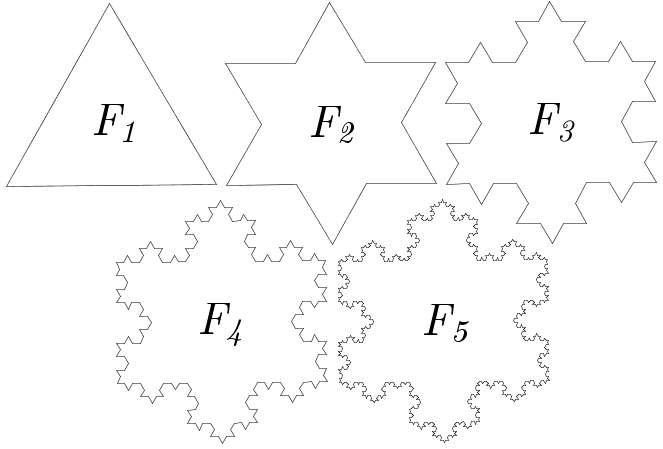
\includegraphics[height=8cm]{chap02_flocons}
\end{center}
\end{chistoire}

\end{document}